\chapter{直线运动}\label{chapter-rectilinear-motion}

\section{机械运动}
 我们在初中学过,一个物体相对于另一个物体的位置变
化叫做\textbf{机械运动},简称运动.在自然界中没有不动的物体.房
屋、桥梁、树术、山岭等总在原地不动,我们说它们是静止的.
其实它们是随着地球一起运动的,不但地球在运动,太阳在
银河系中也是运动的.小到原子和分子,大到宇宙中的天体,
一切物体都在运动,机械运动是宇宙中最普遍的现象.

\subsection{参照物} 

既然一切物体都在运动,我们研究一个物体的
运动时,就必须选取另外的物体作为参照,事先假定这个另外
的物体是不动的,这样才能进行研究.我们说房屋、桥梁等是
静止的,行驶的汽车是运动的,这是选取地面作为参照来说
的;房屋、桥梁等对地面来说位置没有发生变化,行驶的汽车
对地面来说位置发生了变化.坐在行驶的火车车厢里的乘客
认为自己是静止的,在车厢里走动的乘务员是运动的,这是
选取车厢作为参照来说的;乘客对车厢来说位置没有发生变
化,乘务员对车厢来说位置发生了变化.研究物体的运动时,
选来作为参照的另外的物体,叫做\textbf{参照物}.

    原则上,研究一个物体的运动时,参照物是可以任意选取
的.观察在河里游泳的人的运动,可以选择河岸作参照物,也
可以选择在河上航行的船只作参照物.研究天体的运动时,可
以取地球作参照物,也可以取太阳作参照物.但是,实际选取
参照物时,往往要考虑研究问题的方便,使运动的描述尽可能
简单.例如,研究太阳系的行星运动,太阳是最理想的参照物.
研究地面上物体的运动,一般说来取地面做参照物比较方便.

\subsection{平动和转动} 
 物体的运动一般是比较复杂的,但是最基
本的运动只有两种:平动和转动.

    从桌内拉出抽屉的时候,抽屉各部分的运动轨迹完全相
同,也就是说,各部分的运动完全相同.这样的运动就是\textbf{平
动}.打桩时重锤的下落运动,汽缸里活塞的运动,车床上车刀
(图~\ref{fig_A_2-1})的运动,在直铁轨上行驶的火车车厢的运动,都是平
动.
\begin{figure}[htbp]
\centering
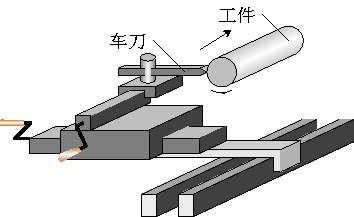
\includegraphics{fig/A/2-1.pdf}
\caption{车床上车刀的平动和工件的转动}\label{fig_A_2-1}
\end{figure}

    物体的平动不一定都沿着直线进行,也可以沿曲线进行,
图~\ref{fig_A_2-2} 所示的铅笔的平动就是沿着曲线进行的.
\begin{figure}[htbp]
\centering
\begin{minipage}[t]{0.48\textwidth}
\centering
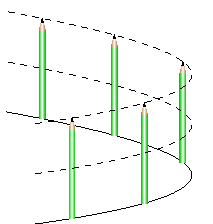
\includegraphics{fig/A/2-2.pdf}
\caption{沿曲线进行的平动}\label{fig_A_2-2}
\end{minipage}
\begin{minipage}[t]{0.48\textwidth}
\centering
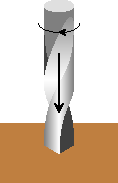
\includegraphics{fig/A/2-3.pdf}
\caption{钻头在工作中同时做平动和转动}\label{fig_A_2-3}
\end{minipage}
\end{figure}
    
    推动石磨的时候,磨盘上的各部分都围绕着通过中心
的轴线做圆周运动.这样的运动就是\textbf{转动}.脱粒机的滚筒的
运动,机器上飞轮的运动,车床上工件的运动(图~\ref{fig_A_2-1}),都是
转动.


    在很多情况下,物体同时做平动和转动.钻头在工作的
时候(图~\ref{fig_A_2-3}),车轮在路上滚动的时候,螺栓在拧入螺母中的
时候,都是同时做平动和转动的.

\section{质点}
    物体都具有大小和形状,在运动中物体各点的位置变
化一般说来是各不相同的,所以要详细描述物体的运动,并不
是一件简单的事情.可是,在某些倩况下,却可以不考虑物体
的大小和形状,而使问题简化.在这些情形下,我们可以把物
体看作一个有质量的点,或者说用一个有质量的点来代替整
个物体,用来代替物体的有质量的点叫做\textbf{质点}.

    在什么情况下可以把物体当作质点,这要看具体情况而
定.举例来说,当我们研究地球的公转时,由于地球的直径(约
$1.3\times 10^4$千米)比地球和太阳之间的距离(约$1.5\times 10^8$千米)
要小得多,因而可以忽略地球的大小和形状,把它当作质点,
可是研究地球的自转时,我们却不能忽略地球的大小和形状,
当然不能把地球当作质点了.

    一个平动的物体,它的各个部分的运动情况都相同,它的
任何一点的运动都可以代表整个物体的运动.在这种情况
下,也可以把整个物体当作质点来看待.一辆在直公路上行
驶的汽车,车身上各部分的运动情况相同,当我们把汽车作为
一个整体来研究它的运动的时侯,就可以把汽车当作质点.当
然,假如我们需要研究汽车的轮胎的运动,由于轮胎的各部分
的运动情况不相同,那就不能把它看作质点了.

    今后我们研究的物体,除非涉及到转动,一般都可以看作
质点.

    任何物体都具有一定的大小和形状,因此质点这个概念
是一种科学的抽象,是一种理想化的模型.我们研究物体的
运动,像研究其他物理现象一样,不能主次不分.如果物体的
大小和形状在所研究的现象中起的作用很小,可以忽略不计,
我们就可以把物体看作是一个没有大小和形状的理想物体,
即质点.这种研究问题的方法,在物理学中是常常用到的.

    研究物体的运动,第一步是要知道物体是怎样运动的,也
就是知道物体的运动情况.物体在运动过程中,它的位置和
速度不断随时间而变化,如果我们知道了物体在任一时刻的
位置和速度,就表示我们知道了物体的运动情况.这一章我
们就围绕着这个要求来研究直线运动.

 \subsection*{练习一}
\begin{enumerate}
\item 两辆在公路上直线行驶的汽车,它们的距离保持不
变.试说明用什么样的物体做参照物,两辆汽车都是静止的,
用什么样的物体做参照物,两辆汽车都是运动的.能否找到
这样一个参照物,一辆汽车对它是静止的,另一辆汽车对它是
运动的?为什么?

\item 小孩从滑梯上滑下,钢球沿斜槽滚下,石块从手中
落下,这些物体中哪些是做平动的?

\item 研究自行车轮的转动,能不能把自行车当作质点?研
究在马路上行驶的自行车的速度,能不能把自行车当作质点?
\end{enumerate}

\section{位置和位移}
    研究质点的运动,首先要知道怎样确定质点的位置.质
点的位置可以采取在数学中学过的建立坐标系的方法来确
定.质点做直线运动时,我们可以取这条直线为坐标轴($x$
轴),在轴上任选一点$O$为原点,规定好坐标轴的正方向和单
位,质点的位置由它的位置坐标,即一个带有正负号的数值,
就可以完全确定了.比如我们要确定一辆行驶在北京长安街
上的汽车的位置,我们可以取$x$轴表示长安街的东西方向,$x$
轴的正方向指东,并且取天安门前的旗杆作为坐标原点,那么
汽车的位置就由它的坐标完全确定了.汽车的坐标是1千
米,表示它在旗杆以东1千米处;汽车的坐标是$-2$千米,表
示它在旗杆以西2千米处(图~\ref{fig_A_2-4}).
\begin{figure}[htp]
    \centering
    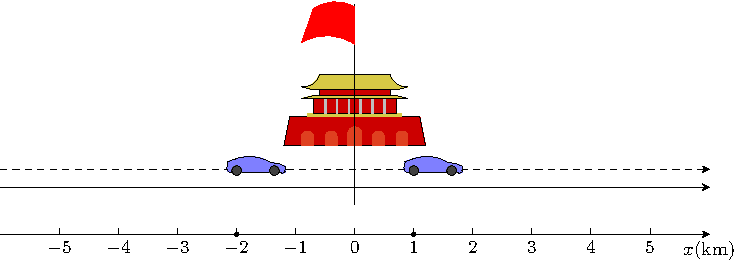
\includegraphics{fig/A/2-4.pdf}
    \caption{}\label{fig_A_2-4}
\end{figure}

    质点在运动过程中,它的位置随时间不断变化,怎样表
示质点的位置变化呢?物理学中用一个叫做位移的物理量来
表示质点位置的变化.设质点原来在$A$点,经过一段时间沿
轨迹$ACB$运动到$B$点(图~\ref{fig_A_2-5}).从初位置$A$指向末位置$B$
作线段$AB$,用它就可以描述质点的位置变化,我们把它叫做
质点的位移.$AB$的长度,即位移的大小,表示出位置变化的
大小;$AB$的方向,即位移的方向,表示出位置变化的方向.位
移既有大小,又有方向,是一个矢量.

\begin{figure}[htp]
    \centering
    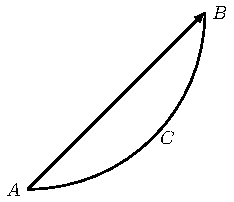
\includegraphics{fig/A/2-5.pdf}
    \caption{}\label{fig_A_2-5}
\end{figure}
\begin{figure}[htp]
    \centering
    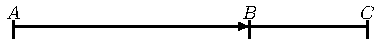
\includegraphics{fig/A/2-6.pdf}
    \caption{}\label{fig_A_2-6}
\end{figure}

    位移和路程是两个不同的物理量.路程是指质点所通过
的实际轨迹的长度,只有大小,没有方向,是标量.在图~\ref{fig_A_2-5} 
中,质点的位移是线段$AB$,而路程是曲线弧$\wideparen{ACB}$的长度,即
使在直线运动中位移的大小也不一定等于路程.图~\ref{fig_A_2-6} 表示
做直线运动的质点从初位置$A$经过$B$运动到$C$,然后从$C$返
回,运动到末位置$B$,这时质点的位移是线段$AB$,而路程是
线段$AC$的长度加上线段$BC$的长度.只有做直线运动的质
点始终向着同一个方向运动时,位移的大小才等于路程.可
见,位移矢量一般并不表示运动的实际轨迹和路程,而是表示
位置的变化.

    在物理学中,通常用$s$代表位移.质点做直线运动时,位
移可以用末位置的坐标$x$和初位置的坐标$x_0$表示出来:
\[s=x-x_0\]
\begin{figure}[htp]
    \centering
    \begin{subfigure} {1\linewidth} 
		\centering
		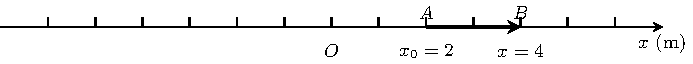
\includegraphics{fig/A/2-7a.pdf} 
		\caption{}\label{fig_A_2-7a} 
	\end{subfigure} 
	\\
    \begin{subfigure} {1\linewidth} 
        \centering
        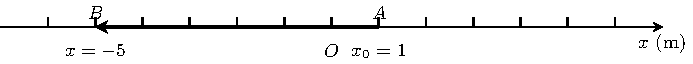
\includegraphics{fig/A/2-7b.pdf} 
        \caption{}\label{fig_A_2-7b} 
    \end{subfigure} 
    \caption{位移的坐标表示}\label{fig_A_2-7}
\end{figure}

这就是说,位移的数值等于末位置的坐标$x$减去初位置
的坐标$x_0$.在图~\ref{fig_A_2-7} 中,$A$点表示初位置,$B$点表示未位置.图甲
中,$s=x-x_0=4-2=2$米,位移是正值,它的大小
是2米,方向与坐标轴的正方向相同.图乙中,$s=x-x_0=-5-1=-6$
米,位移是负值,它的大小是6米,方向与
坐标轴的正方向相反.可见,在直线运动中,用一个带有正
负号的数值就可以把位移矢量的大小和方向都表示出来.

    为了方便,在计算位移时常常取初位置为坐标原点,即
$x_0=0$.这时质点的位移就可以用末位置的坐标来表示:
\[s=x\]

\subsection*{练习二}
\begin{enumerate}
  \item   质点做什么运动,位移的大小才等于路程?
  \item  图~\ref{fig_A_2-6} 表示做直线运动的质点从初位置$A$经过$B$运
  动到$C$,然后从$C$返回,运动到末位置$B$.设$AB$长7米,$BC$长
  5米.求质点的位移的大小和路程.
  \item 在图~\ref{fig_A_2-4} 中,汽车初位置的坐标是$-2$千米,末位置的
  坐标是1千米.求汽车的位移的大小和方向.
  
\end{enumerate}


\section{匀速直线运动~~速度}
    现在我们开始研究物体的运动.从哪里来开始呢?也许从
最常见的运动开始比较好吧!一片树叶从树枝上落下是一种
很常见的运动,可是仔细观察一下,却发现这种运动很复杂,
树叶忽左忽右,有时还发生翻转等,不便于研究.物理学中
研究问题常常是从最简单的现象着手.因此,我们从最简单
的运动即匀速直线运动来开始对运动的研究.

    火车在平直的铁路上行驶,如果它每分钟的位移是900
米,每秒钟的位移是15米,也就是在相等的时间内位移相等,
这列火车所做的运动就是\textbf{匀速直线运动}.

\textit{物体在一条直线上运动,如果在相等时间里的位移相等,
这种运动就叫做匀速直线运动}.匀速直线运动有时简称为\textbf{匀速运动}.

    飞机在天空中匀速飞行,轮船在海洋上匀速航行,它们的
运动虽然都是匀速运动,但还是有区别的.在相同的时间里,
飞机的位移大,轮船的位移小,即飞机飞得快,轮船走得慢.在
物理学中怎样来表示匀速运动的快慢呢?在匀速运动中,物
体在相等时间内的位移相等,因此,如果物体在时间$t$内的位
移是$s$,在$2t$时间内的位移一定是$2s$,在$3t$时间内的位移
一定是$3s$,等等.可见匀速运动的位移和时间的比值是一个
恒量,不随时间而改变.这个比值越大,表示物体运动得越
快.

\textit{在匀速直线运动中,位移和时间的比值,叫做匀速直线
运动的}\textbf{速度}.

如果做匀速运动的物体在时间$t$内的位移是$s$,速度$v$
就可以用下式来表示:
\[v=\frac{s}{t} \]

由上式可以看出,速度在数值上等于单位时间内位移的
大小.

    速度的单位有厘米/秒,米/秒,千米/小时等.在国际单
位制中,速度用米/秒($\Ums$)作单位.

    速度不但有大小,而且有方向,是矢量.速度矢量的方向
就是物体位移的方向.在匀速直线运动中,计算时通常取位
移方向作为正方向,速度是正值.

从速度的公式$v=s/t$
可以得到
  \[s=vt \]

这个公式叫做匀速运动的\textbf{位移公式},它表示出匀速运动
的位移跟时间的关系:位移跟时间成正比.利用这个公式,只
要知道了速度$v$,就可以求出做匀速运动的物体在任何时间
内的位移.如果还知道物体的初位置,就可以确定做匀速运
动的物体在任一时刻所在的位置.

这里提到了时间和时刻,顺便说一下它们的区别.我们说.
现在是9时10分,这是指的时刻.我们说从9时10分到9
时50分,这是指的一段时间,这段时间是40分钟.如果用坐
标轴来表示时间,那么时刻相当于轴上的一点,时间相当于轴
上的一段距离.坐标轴原点的时刻为零,$t=0$,表示从这一时
刻开始计时.

\subsection*{练习三}

\begin{enumerate}
    \item 光在真空中沿直线传播的速度为$3.0\times 10^8\Ums$.
\begin{enumerate}
    \item 一光年(光在一年中传播的距离)有多少千米?
    \item 最靠近我们的恒星(半人马座$\alpha$星)离我们$4.0\times 10^{13}$千米,它发出的光要多长时间才到达地球?
\end{enumerate}    
\item  在技术上常用$\UkmhA$作速度的单位.试求$1 \Ums$合多少$\UkmhA$.
\item 光在空气中的速度可以认为等于光在真空中的速
度.声音在空气中的速度是340$\Ums$.一个人看到闪电后5
秒听到雷声,打雷的地方离他大约多远?

\end{enumerate}

\section{匀速直线运动的图象}
    物体运动的情况可以用公式来表示,也可以用函数图象
来表示.这一节学习怎样用图象来表示匀速直线运动.

    \subsection{匀速直线运动的位移图象} 
    
    任意选择一个平面直角坐标
系、用横轴表示时间,用纵轴表示位移,画出位移和时间的关
系图线,这种图象叫做\textbf{位移—时间图象},简称为\textbf{位移图象},匀速直线运动的位移$s$
是时间$t$的正比函数$s=vt$.
\begin{figure}[htp]
    \centering
    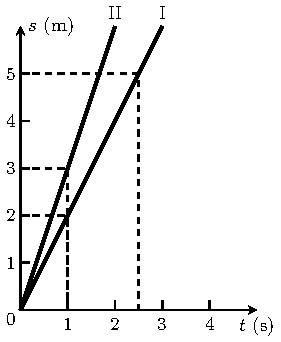
\includegraphics{fig/A/2-8.pdf}
    \caption{匀速运动的位移图象.
    取初位置为坐标原点时,质点的位移等于末位置的坐标,因此这个
    图象也可以叫做质点的位置—时间图象.}\label{fig_A_2-8}
\end{figure}

在初中数学里已经学过,正比函数的图象是一条通过原
点的直线.图~\ref{fig_A_2-8} 中的直线~I是速度为$20 \Ums$的匀速运动
的位移图象,直线II是速度为$v=3 \Ums$的位移图象.


    应用匀速运动的位移图象,我们可以求出物体在任意时
间内的位移.例如从图~\ref{fig_A_2-8} 可以求出,$v=2\Ums$的匀速运动
在2.5秒内的位移是5米,应用位移图象也可以反过来求出
物体通过任一位移所需的时间.


我们还可以从匀速运动的位移图象求出物体的速度.

\begin{figure}[htp]
    \centering
    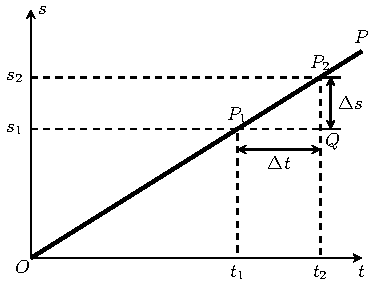
\includegraphics{fig/A/2-9.pdf}
    \caption{匀速运动的速度等
    于位移图线的斜率}\label{fig_A_2-9}
\end{figure}

    在图~\ref{fig_A_2-9} 所示的匀速运动的位移图线$OP$上,任取两点
    $P_1(t_1,s_1)$和$P_2(t_2,s_2)$.用$\Delta t$表示$t_2-t_1$,用$\Delta s$
    表示$s_2-s_1$.
    在直角三角形$P_1QP_2$中,比值
    $\dfrac{\Delta s}{\Delta t}=\dfrac{QP_2}{P_1Q}$越大,
$\angle P_2P_1Q$也越大,直线$OP$就越陡.所以我们把
$\Delta s/\Delta t$叫做直线的\textbf{斜
率},用字母$k$来表示.$\Delta s$是物体在$\Delta t$内的位移,比
值 $\Delta s/\Delta t$
是匀速运动的速度$v$,因此
\[k=\frac{\Delta s}{\Delta t}=v\]

这样,我们得到结论:在匀速直线运动中,位移图线的斜
率等于运动的速度.在同一个坐标平面上,斜率越大,即直线
越陡,表示速度越大.

 
\subsection{匀速直线运动的速度图象} 

匀速直线运动的速度和时间
的关系,也可以用图象来表示.

在平面直角坐标系中,用横轴表示时间,用纵轴表示速
度,画出速度和时间关系的图线,这种图象叫做运动的\textbf{速度—时间图象},简称为\textbf{速度图象}.匀速运动的速度不随时间改变,
它的速度图象是一条与横轴平行的直线,图~\ref{fig_A_2-10} 中的两条直
线I和II分别表示$v=2$$\Ums$和$v=5$$\Ums$的匀速运动的
速度图象.在同一个坐标平面上,图象的直线在纵轴上的截
距越大,表示速度越大.
\begin{figure}[htp]
    \centering
    \begin{minipage}[t]{0.48\textwidth}
        \centering
        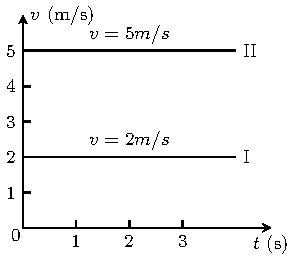
\includegraphics{fig/A/2-10.pdf}
        \caption{匀速运动的速度图象}\label{fig_A_2-10}
    \end{minipage}
    \begin{minipage}[t]{0.48\textwidth}
        \centering
        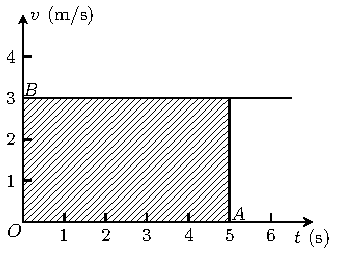
\includegraphics{fig/A/2-11.pdf}
        \caption{由速度图象求位移}\label{fig_A_2-11}
    \end{minipage}
\end{figure}

应用速度图象可以求出质点在任何时间内的位移,设有
一个骑自行车的人以3$\Ums$的速度做匀速运动,速度图象如
图~\ref{fig_A_2-11} 所示.现在来求他在5秒钟内的位移.为了求出位
移,根据公式$s=vt$,必须用时间和速度相乘,也就是用横轴
上的线段$OA=5$秒和纵轴上的线段$OB=3$$\Ums$相乘.图~\ref{fig_A_2-11} 
中画有斜线的长方形的“面积”,表示的就是这个位移的
大小,它的数值是$3 \Ums \times 5 \Us = 15 \Um$,也就是说,位移的数
值等于这个长方形“面积”的数值.这里我们把“面积”一词打
上引号,是因为这个长方形的底的单位是秒,高的单位是$\UmsA$,这个面积的单位是$\UmsA \times \UsA= \UmA $,而不是$ \UmqA $.

\subsection*{练习四}
\begin{figure}[htp]
    \centering
    \begin{minipage}[t]{0.48\textwidth}
        \centering
        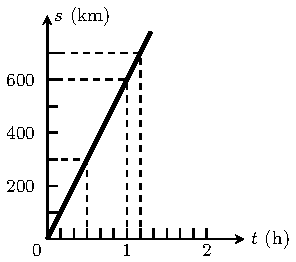
\includegraphics{fig/A/2-12.pdf}
        \caption{}\label{fig_A_2-12}
    \end{minipage}
    \begin{minipage}[t]{0.48\textwidth}
        \centering
        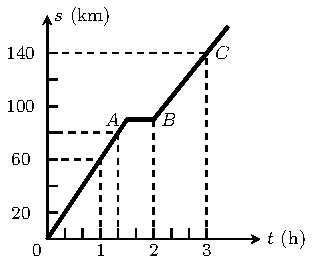
\includegraphics{fig/A/2-13.pdf}
        \caption{}\label{fig_A_2-13}
    \end{minipage}
\end{figure}

\begin{enumerate}
\item 
图~\ref{fig_A_2-12} 是一架民航飞机的位移图象.从这个图象求出
\begin{enumerate}
    \item 飞机在30分钟内的位移;
    \item 飞行700千米所用的时间;
    \item 飞行速度并画出速度图象.
\end{enumerate}

\item  
图~\ref{fig_A_2-13} 是一辆火车运动的位移图象.线段$OA$和$BC$
所表示的运动,哪个速度大?各等于多大?线段AB与横轴平
行,表示火车做什么运动?速度是多大?火车在3小时内的位移
是多少?通过80千米用多长时间?画出火车的速度图象.


\item  
有两个物体,从同一点开始向相同方向做匀速运动,
速度分别是3$\Ums$和5$\Ums$,在同一个坐标平面上画出它们
的位移图象和速度图象,并根据这两种图象分别求出它们在5
秒内的位移.

\end{enumerate}


\section{变速直线运动~~平均速度~~即时速度}
    \subsection{变速直线运动}
    
    我们日常看到的直线运动,往往不是匀
速的.飞机起飞的时候,运动越来越快,在相等时间里的位移
是不相等的.火车进站的时候,运动越来越慢,在相等时间里
的位移也是不相等的.

\textit{物体在一条直线上运动,如果在相等时间里的位移不相等,这种运动就叫做\textbf{变速直线运动}}.变速直线运动有时简称为\textbf{变速运动}.

\subsection{平均速度}

变速运动的物体在相等的时间里的位移不
相等,所以它没有恒定的速度.那么,我们怎样来描述它的快
慢呢?粗略的办法是把它看作匀速运动.一列火车,半小时
内走了28千米,尽管它的运动时快时慢,我们仍然可以设想
火车在这半小时内是匀速运动的,这样它的速度就是$56 \Ukmh$.这个$56 \Ukmh$,就是火车在这半个小时内的\textbf{平
均速度}.

\textit{在变速直线运动中,运动物体的位移和所用时间的比值,
叫做这段时间里的平均速度}.
如果用$\bar v$来表示平均速度,那么
\[\bar v=\frac{s}{t}\]

平均速度的数值跟在哪一段时间内计算平均速度有关,
上面讲的那列火车,如果在第一个十分钟走了8千米,在第二
个十分钟走了9千米,在第三个十分钟里走了11千米,它在
三个十分钟里的平均速度就分别是48$\Ukmh$,54$\Ukmh$,66$\Ukmh$.可见,火车半小时内的平均速度虽然是
56$\Ukmh$,但在每个十分钟里的平均速度却是不同的,它
的运动逐步加快.

\subsection{即时速度}
平均速度只能粗略地描述做变速运动的物体
的运动情况,要精确地描述变速直线运动,还需要知道物体在
每一时刻(或位置)的运动速度.运动物体在某一时刻(或某
一位置)的速度,叫做\textbf{即时速度}.

物体在某一时刻或某一位置的速度的意义是什么呢?图~\ref{fig_A_2-14} 
表示一辆做变速运动的汽车.我们要确定汽车经过$A$点
时的即时速度.从$A$起取一小段位移$AA_1$,求出在这段位移上
的平均速度,这个平均速度可以近似地表示汽车经过$A$点的
快慢程度.从$A$起所取的位移越小,比如依次取位移$AA_2$、$AA_3$
等,所得的平均速度用来表示汽车经过$A$点的快慢程度就
越精确.当位移足够小时,
或者说时间足够短时,所得
的平均速度就等于汽车经过$A$点的即时速度了.

这里所说的“足够短”,应该怎样理解呢?原来,做变速运
动的物体的速度总是连续变化的,位移取得越小,或者说时间
取得越短,在这段时间内速度的变化就越小.时间足够短时,
测量仪器已经分辨不出变速运动和匀速运动的差别,可以认
为这一小段时间的运动是匀速的.这时,即使进一步缩短所
取的时间,测得的平均速度也不会有什么变化,这个平均速度
就等于即时速度.

\begin{figure}[htp]
    \centering
    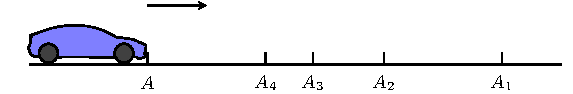
\includegraphics{fig/A/2-14.pdf}
    \caption{}\label{fig_A_2-14}
\end{figure}

用数学语言可以更为精确地表达上面所讲的意思.在图~\ref{fig_A_2-14} 
中从$A$起取一小段位移$\Delta s$,求出这小段位移内的平均
速度$\Delta s/\Delta t$, 当$\Delta t$\textbf{趋近于}零时,平均速度\textbf{趋近于}某一固定数
值—一极限值,这个极限值就是汽车经过$A$点的即时速度.

    即时速度既有大小,又有方向,是矢量.在直线运动中,
即时速度的方向就是物体经过该点时的运动方向.即时速度
的大小叫做\textbf{即时速率},简称\textbf{速率},它是一个表示物体运动快慢
程度的标量,在某些问题中,如果只需考虑即时速度的大小,
可以用速率的概念.

    在匀速运动中,知道了速度,根据位移公式就可以确定运
动物体在任一时刻的位置,在变速运动中,怎样确定物体在
任一时刻的位置和速度呢?

    一般地讨论这个问题过于复杂,下面我们只就最简单的
变速运动来研究这个问题.

\subsection*{练习五}

\begin{enumerate}
    \item 一辆汽车,起初以30$\Ukmh$的速度匀速行驶了30千米,然后又以60$\Ukmh$的速度匀速行驶了30千米.一位
    同学认为这辆汽车在这60千米中的平均速度是$1/2\cdot(30 \Ukmh+60\Ukmh)=45\Ukmh$.这个结果对不对?
    \item 骑自行车的人沿着坡路下行,在第1秒内通过1米,
    第2秒内通过3米,在第3秒内通过5米,在第4秒内通过7米.求
    最初两秒内、最后两秒内以及全部运动时间内的平均速度.
    \item 在一个速度是$v$的匀速直线运动中,各段时间内的
    平均速度以及整个运动的平均速度各是多大?每一时刻的即
    时速度是多大?
    \item 火车以70$\Ukmh$的速度经过某一路标,子弹以
    600$\Ums$的速度从枪筒射出.这里指的是什么速度?
    
\end{enumerate}


\section{匀变速直线运动~~加速度}
    \subsection{匀变速直线运动}
    
    伽利略(1564 $\sim$1642)是首先认真研究
变速运动的物理学家.伽利略就是从最简单的变速运动着手
的.他设想,最简单的变速运动的速度应该是均匀变化的.
但是,速度的变化怎样才算均匀呢?他考虑了两种可能:一种
是速度的变化对时间来说是均匀的,即经过相等的时间,速度
的变化相等;另一种是速度的变化对路程来说是均匀的,即
经过相等的路程,速度的变化相等.伽利略断定第一种方式最
为简单,并且用实验研究了斜面上滚下来的铜球,证明这种运
动方式在自然界中是的确存在的.这种运动,就是我们现在
要研究的匀变速直线运动.

\textit{在一条直线上运动的物体,如果在相等的时间里速度的
变化相等,
物体的运动就叫做\textbf{匀变速直线运动}},或者简称为\textbf{匀变速运动}.

举例来说,一个做直线运动的物体,在某一时刻它的速度
是3$\Ums$,过了1秒钟变成4$\Ums$,再过1秒钟变成5$\Ums$,
它的速度每秒钟增加1$\Ums$,这个物体做的就是匀变速运
动.又如一个做直线运动的物体,在某一时刻它的速度是
8$\Ums$,过了1秒钟变成6$\Ums$,再过1秒钟变成4$\Ums$,
它的速度每秒钟减小2$\Ums$,这个物体做的也是匀变速运
动.

    常见的许多变速运动实际上并不是匀变速运劝,可是不
少变速运动很接近于匀变速运动,可以当作匀变速运动来处
理.石块从不高的地方下落的运动,发炮时炮弹在炮筒里的运
动,火车、汽车等交通工具开动后一段时间内的运动,竖直抛
出的石块向上的运动,交通工具在停止前的一段运动,都可以
看作是匀变速运动.

\subsection{加速度}
不同的匀变速运动,即时速度的变化有快有慢,
汽车开动时,它的速度在几秒钟内从零增加到几十米每秒.而
发炮时,炮弹的速度在千分之几秒内就从零增加到几百米每
秒.显然汽车的速度增加得慢,炮弹的速度增加得快.火车
进站时速度减小得慢,而汽车在急刹车时速度减小得快.怎样
来表示速度变化的快慢呢?为此,物理学中引入了一个新的
物理量——加速度.

在匀变速直线运动中,在相等的时间里速度的变化相等,
时间$t$增加几倍,速度的变化$v_t-v_0$也增加几倍,因而速度
的变化跟发生这个变化所用的时间的比值是一个恒量,不随
时间而改变.这个比值越大,表示速度变化得越快.

\textit{在匀变速直线运动中,速度的变化和所用的时间的比值,
叫做匀变速直线运动的加速度}.

用$v_0$表示运动物体开始时刻的速度(初速度),用$v_t$表
示经过一段时间$t$的速度(末速度),用$a$表示加速度,那么,
\[a=\frac{v_t-v_0}{t}\]

由上式可以看出,加速度在数值上等于单位时间内速度
的变化.

    加速度的单位是由时间的单位和速度的单位确定的.在
国际单位制中,时间的单位是秒,速度的单位如果用$\Ums$、加
速度的单位就是$\Ums$$^2$,读作米每二次方秒.速度的单位如
果用$\Ucms$,加速度的单位就是$\Ucmsq$.

    加速度不但有大小,而且有方向,因此是矢量.在直线运
动中,取开始运动的方向作为正方向时,$v_0$为正值.在这种情
形下,如果$v_t>v_0$,$a$是正值,表示加速度的方向与初速度的
方向相同;如果$v_t<v_0$,$a$是负值,表示加速度的方向与初速
度的方向相反.

    在匀变速直线运动中,加速度矢量是恒定的,大小和方向
都不改变,因此匀变速直线运动也就是加速度矢量恒定的运
动.

\begin{example}
做匀变速运动的火车,在20秒内速度从10$\Ums$增加到15$\Ums$,加速度是多大?汽车急刹车时做匀变速
运动,在2.0秒内速度从10$\Ums$减小到零,加速度是多大?
\end{example}

\begin{solution}
取初速度的方向作为正方向.火车的加速度$a_1$是
\[a_1=\frac{v_t-v_0}{t}=\frac{10 \Ums -10\Ums}{20\Us}=0.25\Umsq \]
加速度$a_1$是正值表示加速度的方向跟速度的方向相同.这
一结果表示火车的速度每经过1秒就增加$0.25 \Ums $.

汽车的加速度$a_2$是
\[a_2=\frac{v_t-v_0}{t}=\frac{0\Ums-10\Ums}{2.0\Us }=-5.0\Umsq  \]
加速度$a_2$是负值表示加速度的方向跟速度的方向相反.这
一结果表示汽车的速度每经过1秒就减小5.0$\Ums$.

\end{solution}

\section*{阅读材料:速度和加速度的区别}
    速度和加速度是描述运动的两个重要的物理量.清楚地
理解它们的意义及其区别,才能很好地掌握本章所讲的内容.
这里,我们就谈一下这个问题.

    速度是描述物体运动快慢的物理量,或者说描述位置变
化快慢的物理量.速度越大,表示运动得越快,或者说位置变
化得越快.加速度是描述速度变化快慢的物理量,加速度越
大,表示速度变化得越快.

    速度等于位移和时间的比值,因而速度是位置对时间的
变化率.加速度等于速度的变化和时间的比值,因而加速度
是速度对时间的变化率.所谓某一个量对时间的变化率,是
指单位时间内该量变化的数值.变化率表示变化的快慢,不
表示变化的大小.

    速度的大小决定于位移和发生这段位移所用的时间,位
移大,速度并不一定大,因为发生这段位移所用的时间可能很
长.加速度的大小决定于速度变化的大小和发生这一变化所
用的时间,而不决定于速度本身的大小以及速度变化的大小.
汽车起动时虽然速度很小,加速度却较大.汽车在正常行驶
时,速度很大,加速度却很小,甚至为零.

    速度和加速度都是矢量.在直线运动中,速度的方向就
是位移的方向,而加速度的方向可能跟速度方向相同,也可能
跟速度方向相反.当加速度的方向跟速度方向相同时,速度
在增大;当加速度的方向跟速度方向相反时,速度在减小.

\subsection*{练习六}
\begin{enumerate}
\item  加速度为零的运动是什么运动?
\item  有人说:速度越大表示加速度也越大.这话对吗?为什么?
\item  汽车的加速性能是反映汽车质量的重要标志.汽车
从一定的初速度$v_0$加速到一定的末速度$v_t$,用的时间越少,表
明它的加速性能越好.下表是三种型号汽车的加速性能的实
验数据,求它们的加速度.
\begin{center}
\vspace{0.3cm}
\begin{tabular}{ccccc}
\toprule
汽车型号 & 初速度$v_0$ & 末速度$v_t$ & 时间$t$ & 加速度$a$\\
& (km/h)& (km/h)& (s)& (m/s$^2$)\\
\midrule
某型号高级轿车& 20& 50& 7 \\
某型号4吨载重汽车& 20& 50& 38\\
某型号8吨载重汽车& 20& 50& 50\\
\bottomrule
\end{tabular}
\vspace{0.3cm}
\end{center}

\item   以18$\Ums$的速度行驶的火车,制动后经15秒停止,
求火车的加速度.

\end{enumerate}

\section{匀变速直线运动的速度}

\subsection{匀变速运动的速度}

做匀速运动的物体,在相等的时间
里发生的位移都相等,如果知道了位移和时间的比值,即知道
了速度,就可以确定位移和时间的关系;如果还知道初位置,
就可以知道任一时刻的位置.跟这类似,在匀变速运动中,在
相等的时间里速度的变化都相等,如果知道了速度的变化和
时间的比值,即知道了加速度,就可以确定速度的变化和时间
的关系;如果还知道初速度,就可以知道任一时刻的速度.

    前一节里讲过,匀变速运动的加速度公式是
\[a=\frac{v_t-v_0}{t} \]
把这个公式变形,就得到匀变速直线运动的\textbf{速度公式}
\[v_t=v_0+at \]

    这个公式表示出匀变速运动的即时速度是怎样随着时间
而变化的.根据这个公式,如果已经知道做匀变速运动的物
体的初速度和加速度,就可以求出物体在任一时刻的即时速
度.

    如果匀变速运动的初速度为零,即$v_0=0$,上式就简化成
下式:
\[v_t=at \]


\begin{example}
汽车紧急刹车后加速度的大小是6.5$\Umsq$,
如果必须在2.0秒内停下来,汽车行驶的最大允许速度是多
少$\Ukmh$?
\end{example}

\begin{solution}
    汽车必须在2.0秒内停下来,这就要求它最迟在2秒末
速度变为零,即$v_t=0$.加速度$a$和运动的时间都是已知的,
只要求出初速度$v_0$,就得到汽车的最大允许速度.

    汽车在刹车时,速度越来越小,加速度的方向和速度的方
向相反,取速度的方向为正方向,则加速度为负值,即$a=-
6.5\Umsq$.

    由公式$v_t=v_0+at$解出$v_0$,再把已知量代入得
\[\begin{split}
v_0&=v_t-at\\
&=0-(-6.5 \Umsq )\times 2.0 \Us \\
&=13 \Ums=47 \Ukmh
\end{split} \]
也就是说,汽车的最大允许速度是47$\Ukmh$.
\end{solution}


\subsection{匀变速运动的速度图象}


\begin{figure}[htp]
\centering
    \begin{minipage}[t]{0.48\textwidth}
        \centering
        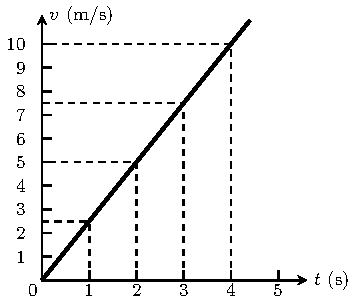
\includegraphics{fig/A/2-15.pdf}
        \caption{$v_0=0 $,$  a=2.5 \Umsq $}\label{fig_A_2-15}
    \end{minipage}
    \begin{minipage}[t]{0.48\textwidth}
        \centering
        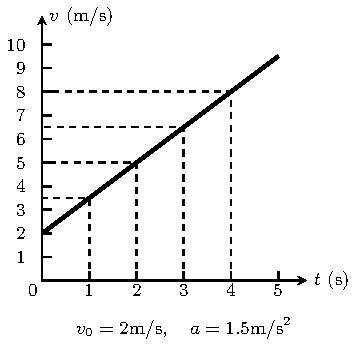
\includegraphics{fig/A/2-16.pdf}
        \caption{$v_0=2 \Ums $,$  a=1.5 \Umsq $}\label{fig_A_2-16}
    \end{minipage}
\end{figure}

\begin{figure}[htp]
    \centering
    \begin{minipage}[t]{0.48\textwidth}
        \centering
        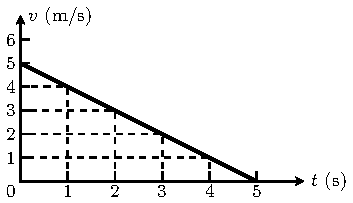
\includegraphics{fig/A/2-17.pdf}
        \caption{$v_0=5 \Ums $,$  a=-1 \Umsq $}\label{fig_A_2-17}
    \end{minipage}
    \begin{minipage}[t]{0.48\textwidth}
        \centering
        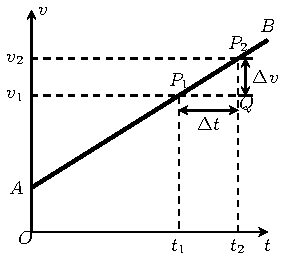
\includegraphics{fig/A/2-18.pdf}
        \caption{速度图线的斜率}\label{fig_A_2-18}
    \end{minipage}
\end{figure}

匀变速运动的速度和时间的关
系,也可以用图象来表示.由于$v_t=v_0+at$是时间$t$的一次
函数,所以匀变速运动的速度—时间图象(简称为速度图象)是
一条直线,图~\ref{fig_A_2-15} 是初速度为零的匀变速运动的速度图象,
图~\ref{fig_A_2-16} 是初速度不为零而加速度为正值的匀变速运动的速
度图象,图~\ref{fig_A_2-17} 是初速度不为零而加速度为负值的匀变速
运动的速度图象.从匀变速运动的速度图象可以求出任意时
刻物体的速度,例如从图~\ref{fig_A_2-15} 可以求出4秒末的速度是10
$\Ums$.从匀变速运动的速度图象也可以求出物体达到某一
速度所需的时间.例如从图~\ref{fig_A_2-16} 可以求出速度达到8$\Ums$
所需的时间是4秒.


    从匀变速运动的速度图象还可以求出加速度.在图~\ref{fig_A_2-18} 所示的速度图象中,用$\Delta t$表示$t_2-t_1$,用$\Delta v$表示$v_2-v_1$,
直线$AB$的斜率$k$为
\[k=\frac{\Delta v}{\Delta t}=a \]
这就是说,匀变速直线运动的速度图线的斜率,等于运动物体
的加速度.在图~\ref{fig_A_2-15} 和图~\ref{fig_A_2-16} 中,$\Delta v=v_2-v_1>0$,斜率$k$为
正值,表示加速度为正值.在图~\ref{fig_A_2-17} 中,$\Delta v=v_2-v_1<0$,斜
率$k$为负值,表示加速度为负值.在同一个坐标平面上,斜率
的绝对值越大,即直线越陡,表示加速度的绝对值越大.

\subsection*{练习七}
\begin{enumerate}
\item 机车原来的速度是36$\Ukmh$,在一段下坡路上加
速度为$0.20\Umsq$,机车行驶到下坡末端,速度增加到54$\Ukmh$.求机车通过这段下坡路所用的时间.
\item 一辆做匀变速运动的汽车,初速度是34$\Ukmh$,
4.0秒末速度变为42$\Ukmh$.如果保持加速度不变,6.0秒
末、7.0秒末的速度是多大?
\item 匀变速运动的加速度是$-4.0\Umsq$.在某一时刻,
速度为$20\Umsq$.试求这一时刻后 4.0秒末和5.0秒末的速度.
\end{enumerate}

\section{匀变速直线运动的位移}
 

\begin{figure}[htbp]
    \centering
    \begin{subfigure} {0.32\linewidth} 
		\centering
		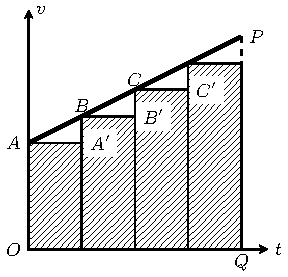
\includegraphics{fig/A/2-19a.pdf}
		\caption{}\label{fig_A_2-19a}
	\end{subfigure}
	\hfill
	\begin{subfigure} {0.32\linewidth} 
		\centering
		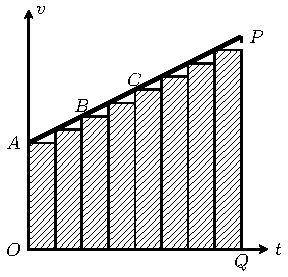
\includegraphics{fig/A/2-19b.pdf} 
		\caption{}\label{fig_A_2-19b}
	\end{subfigure}
	\hfill
	\begin{subfigure} {0.32\linewidth} 
		\centering
		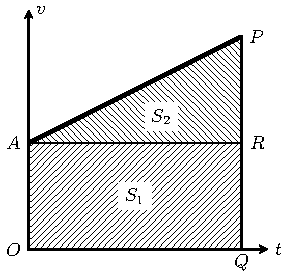
\includegraphics{fig/A/2-19c.pdf} 
		\caption{}\label{fig_A_2-19c}
	\end{subfigure}
    \caption{由匀变速运动的速度图线求位移}\label{fig_A_2-19}
\end{figure}
   匀变速运动的位移又是怎样随着时间而改变的呢?前面
已经讲过,匀速运动的位移可以用它的速度图线和横轴之间
的面积求出来.应用这种方法也可以求出做匀变速运动的物
体的位移.

    图~\ref{fig_A_2-19} 中的直线$AP$是一个做匀变速运动物体的速度
图线.为了求出物体在时间$t$内的位移,我们把时间$t$划分
为许多小的时间间隔,设想物体在每一时间间隔内都做匀速
运动,而从一个时间间隔到下一个时间间隔,物体的速度跳跃
性的突然增加.因此,它的速度图线,由图~\ref{fig_A_2-19a} 中一些平
行于横轴的间断线段$AA' $,$ BB' $,$ CC' $,$ \cdots$组成.我们知道,
匀速运动的位移可以用速度图线和横轴之间的矩形面积来表
示,因此上面设想的物体运动在时间$t$内的位移,其数值等于
图中阶梯状折线$AA'BB'CC'\cdots$下面画有斜线部分的面积.
如某时间的分割再细一些(图~\ref{fig_A_2-19b}),物体速度的跃变发生
得更频繁,它的速度图象就更接近于汽车的真实运动的图象,
阶梯状折线和横轴间画有斜线部分的面积数值,就更接近于
物体的实际位移,这样不断细分下去,当时间间隔分得足够
小时,或
者用数学语言来说,当时间间隔无限细分时
,间断的阶梯线段就趋近于物体的速度图线;阶梯形折线跟
横轴之间的
面积,
也就趋近于速度图线跟横轴之间的面积.这样我们
就得出结论:
匀变速运动的位移可以用速度图线和横轴之间
的面积来表示.
这个结论,不仅对匀变速运动,对一般的变速
运动也是适用的.

由上述讨论可知,所求的匀变速运动的物体在时间$t$内
的位移,等于图~\ref{fig_A_2-19c} 中的梯形$OAPQ$的面积$S$.从图中
可以看出,梯形的面积$S$等于矩形$OARQ$的面积$S_1$和直角
三角形$APR$的面积$S_2$之和:
\[S=S_1+S_2\]
而
 \[\begin{split}
S_1&=OA\times OQ=v_0 t\\
S_2&=\frac{1}{2}AR\times RP=\frac{1}{2}at^2
\end{split}\]
由此可得运动物体在时间$t$内的位移为
\[s=v_0t+\frac{1}{2}at^2 \]

    这个公式叫做匀变速直线运动的\textbf{位移公式}.它表示出匀
变速运动的位移和时间的关系.根据这个公式,如果已经知
道物体的初速度和加速度,就可以求出物体在任何时间内发
生的位移,从而可以确定物体在任一时刻的位置.

    如果匀变速运动的初速度为零,即$v_0=0$,上式就简化成
下式:
\[s=\frac{1}{2}at^2  \]

\begin{example}
以18$\Ums$的速度行驶的汽车,制动后在3.0秒
内前进36米,求汽车的加速度.
\end{example}

\begin{solution}
    在这个问题里,初速度$v_0$、行驶时间$t$和行驶的距离$s$都
是已知的,只要从匀变速运动的位移公式中解出$a$,就可以求
出汽车制动时的加速度.

由公式$s=v_0t+\dfrac{1}{2}at^2$得
\[\begin{split}
a&=\frac{2(s-v_0t)}{t^2}\\
&=\frac{2(36 \Um -18\Ums\times 3.0 \Us )}{(3.0)^2 \Usq}\\
&=-4.0\Umsq
\end{split} \]
    汽车的加速度为$-4.0\Umsq$.负号表明制动产生的加速
度的方向与速度的方向相反.

\end{solution}

\subsection*{练习八}
\begin{enumerate}
\item      钢球在斜槽上做初速度为零的匀变速运动,开始运动
后0.2秒内通过的路程是3.0厘米,1秒内通过的路程是多少?如
果斜面长1.5米,钢球由斜面顶端滚到底端需要多长时间?


\item     飞机着陆后做匀变速运动,速度逐渐减小,已知初
速度是60$\Ums$,加速度的大小是6.0$\Umsq$,求飞机着陆后5.0
秒内通过的路程.


\item     一辆汽车原来匀速行驶,然后1.0$\Umsq$的加速度
加快行驶,经12秒行驶了180米.汽车开始加速时的速度是多
大?


\item     骑自行车的人以5.0$\Ums$的初速度登上斜坡,得到
$-40 \Ucmsq $的加速度,经过10秒钟,在斜坡上通过多长的
距离?

\item    汽车以36$\Ukmh$的速度行驶.刹车后得到的加
速度的大小为4$\Umsq$.从刹车开始,经过3秒钟,汽车通过的
距离是多少?


\end{enumerate}


\section{匀变速运动规律的应用}
    \subsection{两个基本公式}

前两节里我们学习了匀变速直线运动的
速度公式和位移公式:
\begin{align}
v_t&=v_0+at \label{eq-A-2.1} \\
s&=v_0 t+\frac{1}{2}at^2 \label{eq-A-2.2}
\end{align}

    这是两个基本公式,它们表明了匀变速直线运动的规律,
应用它们可以解决匀变速直线运动的各种问题.

    当匀变速运动的初速度为零时,上述两个公式分别简化
为
\begin{align}
v_t&=at \label{eq-A-2.3} \\
s&=\frac{1}{2}at^2 \label{eq-A-2.4}
\end{align}

当$a=0$时,上述基本公式 \eqref{eq-A-2.1} 和 \eqref{eq-A-2.2} 变为匀速运动的公
式:
\[\begin{split}
v_t&=v_0\\
s&=v_0t
\end{split}\]
其中$v_t=v_0$表示物体在任一时刻的速度都与初速度$v_0$相同,
即物体做匀速运动.

    这样,我们看到,一个初速度不为零的匀变速运动,可以
看作是在同一条直线上进行的两个运动合成的:一个是速度
为$v_0$的匀速运动;一个是初速度为零的匀变速运动.关于一
般的运动合成的知识,我们到第\ref{chapter-curvilinear-motion}章再讲解.

\begin{example}\label{exa-A-2.4}
一辆汽车以36$\Ukmh$的速度行驶,司机
看到交通红灯后立即刹车,汽车开始做匀变速运动,加速度的
大小是5.0$\Umsq$.从刹车起到停下来,汽车的位移是多大?
\end{example}

\begin{solution}
    刹车后速度越来越小,加速度为负值,$a=-5.0\Umsq$.
用国际单位制表示各个物理量:$v_0=36\Ukmh=10\Ums$.
汽车最后停下来,$v_t=0$.

    要求出位移可以用公式 \eqref{eq-A-2.2},其中$v_0$和$a$是已知的,$t$是
未知的.要求出$t$可以用公式 \eqref{eq-A-2.1},把$v_t,v_0,a$代入公式就得
到$t$.

从公式 \eqref{eq-A-2.1} 得到
\[t=\frac{v_t-v_0}{a}=\frac{0-10 \Ums}{-5.0\Umsq}=2.0 \Us \]

从公式 \eqref{eq-A-2.2} 得到
\[\begin{split}
s&=v_0t+\frac{1}{2}at^2\\
&=10\Ums \times 2.0 \Us-\frac{1}{2}\times 5.0\Umsq \times 4.0 \Usq\\
&=10 \Um
\end{split} \]


\end{solution}

    一个比较复杂的题目,如这个例题,往往不能只用一个公
式从已知量直接求出未知量.这时可以分步来考虑,从未知
量出发,考虑要求出它需要哪些别的物理量,而这些物理量哪
些是已知的,哪个是未知的;再考虑求出这个未知量又需要知
道哪些物理量.这样考虑下去,直到需要知道的物理量都是
已知量,再进行计算,就可以求出答案来.

\begin{example}\label{exa-A-2.5}
一个滑雪的人,从85米长的山坡上匀变速
滑下,初速度是1.8$\Ums$.末速度是5.0$\Ums$,他通过这段山
坡要多长时间?
\end{example}

\begin{solution}
    要求出时间$t$可以利用公式 \eqref{eq-A-2.1},式中$v_t$和$v_0$
是已知的,$a$是未知的.但是再利用公式 \eqref{eq-A-2.2} 却
不能求出$a$,因为公式 \eqref{eq-A-2.2} 中$s$和$v_0$是已知的,$a$和$t$都是未
知的,怎么办呢?只要我们善于应用学过的代数知识,这个问
题并不难解决.公式 \eqref{eq-A-2.1} 和 \eqref{eq-A-2.2} 组成一个方程组,解这个方程
组正好得出两个未知量$a$和$t$.本题不要求解出$a$,消去$a$,
解出$t$来,就得到了答案.
\begin{align*}
v_t&=v_0+at\\
s&=v_0 t+\frac{1}{2}at^2
\end{align*}

由前式解出$at=v_t-v_0$,代入后式,得到
\[\begin{split}
s&=v_0t+\frac{1}{2}(v_t-v_0)t\\
&=\frac{1}{2}(v_0+v_t)t
\end{split} \]
解出$t$,代入数值得到
\[t=\frac{2s}{v_0+v_t}=\frac{2\times 85 \Um }{1.8\Ums+5.0\Ums}=25 \Us \]
\end{solution}

  我们看到,例题 \ref{exa-A-2.4} 是分步计算的,例题 \ref{exa-A-2.5} 是先进行文字
运算,求出用已知量表达未知量的代数式,然后代入数值计算
的.后一种解法往往比较简便,同学们在熟悉分步计算的同
时,要逐步学会利用文字运算来解题.

    \subsection{两个有用的推论}

从匀变速运动的两个基本公式出发,
我们可以得出两个有用的推论.用这两个推论来解题有时比
较简便.

第一个推论是速度和位移的关系.由公式 \eqref{eq-A-2.1} 解出
\[t=\frac{v_t-v_0}{a} \]
把它代入公式 \eqref{eq-A-2.2},就得到速度和位移的关系式:
\begin{equation}\label{eq-A-2.5}
v^2_t-v^2_0=2as
\end{equation}

当初速度为零时上式变为
\begin{equation}\label{eq-A-2.6}
v^2_t=2as
\end{equation}

    公式 \eqref{eq-A-2.5} 在不知道时间$t$的情况用起来很方便.如例题 \ref{exa-A-2.4} 就可以直接用公式 \eqref{eq-A-2.5} 来求解.由公式 \eqref{eq-A-2.5} 得
\[s=\frac{v^2_t-v^2_0}{2a}=\frac{0-(10\Ums)^2}{2\times (-5.0\Umsq)}=10 \Um\]

    例题 \ref{exa-A-2.5} 不用公式 \eqref{eq-A-2.1} 和 \eqref{eq-A-2.2} 来求解,也可以用公式 \eqref{eq-A-2.1} 和 \eqref{eq-A-2.5} 来求解,希望同学们自己做一下.

    另一个推论是匀变速运动的平均速度.一个做匀变速运
动的物体,在时间$t$内的位移是$s$,它在这段时间内的平均速
度为
\[\bar v=\frac{s}{t} \]
利用基本公式 \eqref{eq-A-2.1} 和 \eqref{eq-A-2.2} 可以求出平均速度$\bar v$跟初速度$v_0$、末
速度$v_t$的关系.把公式 \eqref{eq-A-2.2} 代入上式得到
\[\bar v=v_0+\frac{1}{2}at \]
由公式 \eqref{eq-A-2.1} 解出$at=v_t-v_0$,再代入上式即得
\begin{equation}
\bar v=\frac{1}{2}(v_0+v_t)
\end{equation}

    上式表明:在匀变速运动中,某段时间内的平均速度等于
这段时间的初速度和末速度的算术平均值.要注意这个结论
是利用匀变速运动的公式导出的,所以它只适用于匀变速运
动,对非匀变速运动并不适用.

    这样,我们就可以得到用平均速度来表达的匀变速运动
的位移公式:
\[s=\bar v t=\frac{1}{2} (v_0+v_t)t\]

利用上式来解题有时很方便,如例题 \ref{exa-A-2.4} 用上式解出$t$,
代入数值即得答案.实际上,在例题 \ref{exa-A-2.4} 中我们已经推出了上
式.

    这里我们看到,一个题目往往可以有不同的解法,我们应
该学会用不同的方法来解题,并在此基础上选择简便的办法
来求解.


\section*{阅读材料:伽利略对匀变速运动的研究}
   伽利略是成功地研究匀变速运动的物理学家,他提出了
匀变速运动的定义,并且通过实验证明了他所下的定义符合
常见的变速运动.

    在伽利略的时代,技术比较落后,通过直接测定即时速度
来验证一个物体是否做匀变速运动,是不可能的.但是,伽利
略应用巧妙的数学推理,得出初速度为零的匀变速运动物体
经过的距离与所用时间的平方成正比,即$s\propto t^2$.这样,只要测
出做变速运动的物体经过不同距离所用的时间,就可以验证
这个物体是否在做匀变速运动.这在当时的条件下是可能做
到的.

    伽利略是怎样推出$s\propto t^2$的呢?他的思路大致如下:先由
平均速度$\bar v=s/t$得出$s=\bar v t$.他推断初速度为零、末速度为$v$
的匀变速运动的平均速度$\bar v=v/2$,然后应用这个关系得出
$s=\frac{1}{2} v t$,
再应用匀变速运动的定义$a=v/t$从上式消去$v$,就
导出$s=\frac{1}{2} a t^2$,即$s\propto t^2$.

  伽利略导出这个关系式是很重要的,通过这个关系式和
他提出的匀变速运动的定义,伽利略实际上发现了匀变速运
动的位移和速度的变化规律.

    在推出$s\propto t^2$以后,伽利略着手进行实验验证.他让一个
铜球从斜面上滚下,做了上百次的实验,终于证明了他得出的
匀变速运动规律的正确.在他写的《两种新科学的对话》一书
中,具体介绍了他的实验方法和过程:

\begin{quotation}
    “用一块木料制成长约12库比持\footnote{库比特:古时欧洲用的一种长度单位,相当于45.7厘米.
},宽半库比特,厚三指
的板条,在它的上面刻一条比一指略宽的槽,将这个槽作得很
直,打磨得很光滑,在槽上裱一层羊皮纸(也要尽可能的光
滑),取一个坚硬、光滑并且很圆的铜球放在槽中滚动.将这
个木槽的一端抬高一两个库比特使槽倾斜,就像我要讲的那
样把球放在槽顶让它沿着槽滚下,记录下降的时间,实验要重
复几次,以便使测得的时间准确到两次测定的结果相差不超
过一次脉搏的十分之一.进行这样的操作,肯定了我们的观
察是可靠的以后,将球滚下的距离改为槽长的四分之一,测定
下降的时间,我们发现它准确地等于前者的一半.下一步,我
们用另一些距离进行试验,把全长所用的时间与全长的二分
之一,三分之二,四分之三,或者其它任何分数所用的时间相
比较.像这样的实验,我们重复了整整一百次,结果总是经过
的距离与时间的平方成比例,并且在各种不同坡度下进行实
验,结果也都是如此……”
\end{quotation}

    在这个实验中,最关键的是测量小球滚下所用的时间.伽
利略用的计时器是一架水钟,这是当时最准确的计时装置,对
这种装置,伽利略做了如下的描述:

\begin{quotation}
    “为了测量时间,我们用了一个放在高处的大的贮水容
器,这个容器底部焊着一支直径很小的管子,从它得到很细的
水柱,物体每次沿整个槽长或都分槽长滚下的那段时间里,我
们将流出的水用小杯子分别收集起来,在一个很准确的天平
上称出水的重量;这些重量差及重量比就表明时间差及时间
比.”
\end{quotation}

    短短两段文字,不仅叙述了他所使用的仪器设备和实验
步骤,而且可以看出伽利略的严格的科学态度,伽利略的实
验方法,简单易行,人人都可以做,后人多次重做了他的实验,
都证实了他的结论的正确.

    现在,我们来总结一下伽利略研究匀变速运动的方法和
步骤:
\begin{enumerate}
\item 给出匀变速运动的定义.(假说)
\item 由匀变速运动的定义出发推导出$s\propto t^2$的结果.(推
理)
\item 用实验来检验推导出的给果是否正确,即用斜面小
球实验检验$s/t^2$是否是一个恒量.(实验检验)
\end{enumerate}

伽利略的研究方法对于后来的科学研究具有重大的启蒙
作用.

\subsection*{练习九}
\begin{enumerate}
\item 一个做匀变速运动的物体,初速度为3.0$\Ums$,经过10秒钟,速度变为9.0$\Ums$,它在这10秒钟内的平均速度是多大?
\item 从长3.0米的斜面顶端由静止滚下来的小球,末速度是2.5$\Ums$,求小球滚动所用的时间.
\item 一辆汽车以12$\Ums$的速度行驶,走到一个下坡,得到0.40$\Umsq$的加速度,汽车通过下坡末端的速度是16$\Ums$,这个下坡的长度是多长?
\item 子弹射中墙壁前的速度是400$\Ums$,射到墙壁后穿进墙壁20厘米,子弹在墙内的运动可以看作匀变速运动,求子弹在墙壁内的加速度和运动时间.
\item 试证明做匀变速运动的物体在一段时间内的平均速度等于这段时间的中间时刻的即时速度.

提示:从这段时间开始的时刻计时,在该时刻$t=0$,速
度为$v_0$.设这段时间为$t$,物体在这段时间内发生的位移$s=v_0t +\frac{1}{2}at^2$,利用平均速度的定义式$\bar v=s/t$,求出这段时间内的平均速度,即可证明.不用位移公式,你能不能证明?

注意:这道题中的结论在学生实验中要用到.

\item 做匀变速运动的物体,在各个连续相等时间$t$内的位移分别是$s_1, s_2, s_3,\ldots,s_n$.如果加速度是$a$,试证明:
\[\Delta s=s_2-s_1=s_3-s_2=\cdots=s_n-s_{n-1}=at^2 \]

提示:从第一个$t$秒开始的时刻计时,在该时刻$t=0$,速度为$v_0$,利用位移公式和速度公式可得:
\[\begin{split}
s_1&=v_0t +\frac{1}{2}at^2\\
s_2&=(v_0+at)t +\frac{1}{2}at^2\\
s_3&=(v_0+2at)t +\frac{1}{2}at^2\\
&\cdots\cdots
\end{split} \]

反之,如果在任意连续相等的时间内$s_2-s_1=s_3-s_2=\cdots$,就可以知道这个运动是匀变速运动,这个结论在下
一节和学生实验中要用到.
\end{enumerate}

\section{自由落体运动}
\subsection{自由落体运动}
物体下落的运动是一种常见的而且重
要的运动,挂在线上的重物,如果把线剪断,它在重力的作用下就沿着竖直方向下落.从手中释放的石块,在重力作用下也沿着竖直方向下落,可见物体下落的运动是直线运动.

不同物体的下落运动,情况是否相同呢?

在同一高度同时释放一个金属片和一个纸片,可以看到金属片比纸片下落得快,从这里似乎可以得到结论:物体下落的快慢是由它们的重量决定的,物体越重,下落得越快.十六世纪以前的学者的看法就是这样的.其实这个结论是错误的,它没有考虑空气阻力的影响.纸片比较轻,空气阻力对它的影响比较大,所以才下落得慢.现在我们改变一下实验的作法:把纸片团成一个小纸团,再让它和金属片同时下落.这时纸团受到的空气阻力大为减小,我们可以看到纸团和金属片几乎是同时落地的.
\begin{figure}[htp]
\centering

\includegraphics{fig/A/2-20.pdf}
\caption{在没有空气的空间里,物体下落的快慢相同}\label{fig_A_2-20}
\end{figure}

拿一个长约1.5米,一端封闭,另一端有开关的玻璃筒(图~\ref{fig_A_2-20}).把形状和重量都不同的一些物体,如金属片、小
羽毛、小软木塞、小玻璃球等,放到这个玻璃筒里.如果玻璃筒里有空气,把玻璃筒很快倒立过来以后,这些物体下落的快慢不相同.
如果把玻璃筒里的空气抽出去,把玻璃筒很快倒立过来以后,这些物体下落的快慢就相同了.



物体只在重力作用下,从静止开始下落的运动,叫做\textbf{自由落体运动}.这种运动只有在没有空气的空间里才能发生.在有空气的空间里,如果空气阻力的作用比较小,可以忽略不计,物体的下落也可以看作是自由落体运动.\textit{不同物体的自由落体运动,它们的运动情况是相同的}.

直观告诉人们,自由落体运动是变速运动,但它是不是一种匀变速运动呢?下而用实验来研究这个问题.


\subsection{自由落体加速度}
图~\ref{fig_A_2-21} 是自由落体(小球)的闪光照
片,它是每隔1/30秒的时间拍摄的,由这张照片可以测出小球在各个连续相等时间里的位移.小球最初几个位置比较密集,测量起来误差较大,我们从某个稍大些的位置间隔开始测量.
表 \ref{tab-A-2.1} 第一列是这些间隔的标号,第二列是这些间隔的长度,即小球在各个1/30秒内的位移,第三列是后一间隔的长度减去前一间隔的长度所得的结果.这些值在误差范围内可以认为是相等的,从练习九第6题知道,这表示小球的下落是匀变速运动.可见,\textit{自由落体运动是初速度为零的匀变速运动}.

\begin{figure}[htp]
\centering
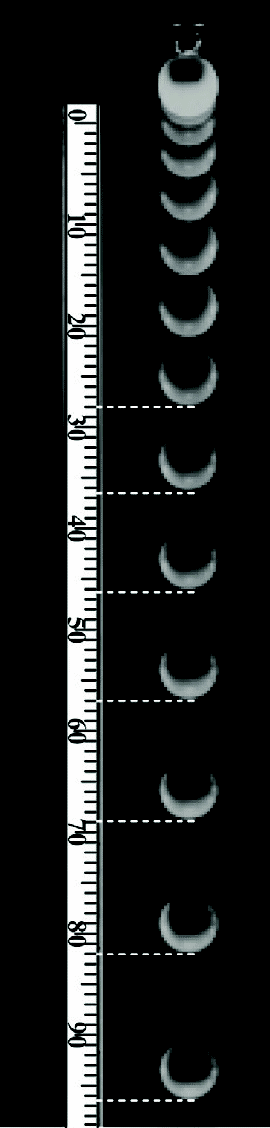
\includegraphics[height=0.93\linewidth, angle=90]{fig/A/2-21.png}
\caption{自由落体的闪光照片}\label{fig_A_2-21}
\end{figure}

不同的自由落体,它们的运动情况相同:它们在做初速度为零的匀变速运动中,在相同的时间内发生相同的位移.由此可以知道,在同一地点,一切物体在自由落体运动中的加速度都相同.这个加速度叫做自由落体加速度,也叫\textbf{重力加速度},通常用$g$来表示.

重力加速度$g$的方向总是竖直向下的,它的大小可以用实验来测定.表 \ref{tab-A-2.1} 中$\Delta s$的平均值是1.08厘米,利用$\Delta s=at^2$就可以求出$g$的数值:
\[\begin{split}
g&=\frac{\Delta s}{t^2}=\frac{1.08}{(1/30)^2} \Ucmsq \\
&=9.7\Umsq
\end{split} \]

\begin{table}
	\centering
	\caption{其中$s$是间隔长度(厘米);$\Delta s$是后一间隔长度减去前一间隔长度(厘米).}\label{tab-A-2.1}
\begin{tabular}{ccc}
\toprule
间隔编号&
$s$&$\Delta s$
 \\
 \midrule
	1&	7.7&	\\
	2&	8.75&	1.05
\\
	3&	9.8&	1.05
\\
	4&	10.85&	1.05
\\
	5&	11.99&	1.16
\\
	6&	13.09&	1.10
\\
	7&	14.18&	1.09
\\
	8&	15.22&	1.04
\\
	9&	16.31&	1.09
\\
	10&	17.45&	1.14
\\
	11&	18.52&	1.07\\
\bottomrule
\end{tabular}

\end{table}



目前国际上取$g=9.80665\Umsq$为重力加速度的标准值,在通常的计算中可以取$g=9.8\Umsq$或$g=980 \Ucmsq $.

根据匀变速运动的公式,可以得出自由落体的速度公式和位移公式
\[\begin{split}
v&=gt\\
s&=\frac{1}{2}gt^2
\end{split}\]
这就是自由落体的运动规律.


\section*{阅读材料:伽利略对自由落体的研究}
古代的学者们认为,物体下落的快慢是由它们的重量决定的,物体越重,下落得越快.生活在公元前四世纪的希腊哲学家亚里士多德最早阐述了这种看法.亚里士多德的论断影响深远,在其后两千多年的时间里,人们一直信奉他的学说.但是这种从表面上的观察得出的结论实际上是错误的,伟大的物理学家伽利略用简单明了的科学推理,巧妙地揭露了亚里士多德的理论内部包含的矛盾.他在1638年写的《两种新科学的对话》一书中指出:根据亚里士多德的论断,一块大石头的下落速度要比一块小石头的下落速度大.假定大石头的下落速度为八.小石头的下落速度为四,当我们把两块石头拴在一起时,下落快的会被下落慢的拖着而减慢,下落慢的会被下
落快的拖着而加快,结果整个系统的下落速度应该小于八,但是两块石头拴在一起,总的重量比大石头的重量还要大,因此重物体比轻物体的下落速度要小.这样,就从重物体比轻物体下落得快的假设,推出了重物体比轻物体下落得慢的结论.亚里士多德的理论陷入了自相矛盾的境地.伽利略由此推断重物体不会比轻物体下落得快.

伽利略认为自由落体运动是一种匀变速运动,但当时他无法用实验直接证实自己的论断,只好求助于间接证明.伽利略先证明了从斜面上滚下的小球是做匀变速运动,然后把结论外推到斜面倾角增大到90$^\circ$的情况,小球将自由下落,成为自由落体.伽利略认为,这时小球仍然会保持匀变速运动
的性质.这种从斜面运动到落体运动的外推,是很巧妙的.不过,用外推法得出的结论,并不一定都是正确的,现代物理研究中也常用外推法,但用这种方法得到的结论都要经过实验的证实才能得到承认.

今天,距离伽利略的时代已有三百多年了,伽利略无法直接用实验来证实的结论,我们已经可以直接用实验来证实了.


\subsection*{练习十}
\begin{enumerate}
	\item 为了测出井口到井里水面的深度,让一个小石块从井口落下,经过2.0秒后听到石块落到水面的声音,求井口到水面的大约深度(不考虑声音传播所用的时间).
\item 一个自由下落的物体,到达地面的速度是39.2$\Ums$,这个物体是从多高落下的?落到地面用了多长时间?
\item 一个物体从22.5米高的地方下落,到达地面时的速度是多大?下落最后1秒内的位移是多大?
\end{enumerate}


\section{竖直上抛运动}
将物体用一定的初速度沿竖直方向向上抛出去,物体所做的运动叫做\textbf{竖直上抛运动}.竖直上抛的物体,在上升过程中,速度越来越小,加速度的方向跟速度的方向相反,是竖直向下的;当速度减小到零的时候,物体上升到最大高度.然后物体从这个高度自由下落,速度越来越大,加速度的方向跟速度的方向相同,也是竖直向下的.如果不考虑空气的阻
力,这两个过程的加速度都是重力加速度$g$.因此,在处理竖直上抛运动的问题时,可以分两步进行计算:上升过程用初速度不为零的匀变速直线运动公式来计算,下降过程用自由落体公式来计算.

由于上升运动和下降运动的加速度矢量是相同的,我们也可以把竖直上抛运动看做是一个统一的匀变速直线运动,而上升运动和下降运动不过是这个统一的运动的两个过程.这样,我们就可以用匀变速运动的速度公式和位移公式来统一讨论竖直上抛运动.在讨论这类问题中,我们习惯上总是
取竖直向上的方向作为正方向,重力加速度$g$总是取绝对值.这样,竖直上抛运动的速度公式和位移公式通常就写做
\[\begin{split}
v_t&=v_0-gt\\
s&=v_0 t-\frac{1}{2}gt^2
\end{split}\]

注意:上述公式中的$t$是从抛出时刻开始计时的,$s$是运动物体对抛出点的位移.

现在我们应用上述公式讨论几个具体问题.
\begin{enumerate}[(1)]
	\item  物体上升的时间
	
	设物体经过时间$t$,上升到最高点,在这一时刻,物体是静止的,由此可得
	\[v_0-gt_1=0 \]
	
	所以物体上升的时间
	\[t_1=\frac{v_0}{g} \]
	
	\item 上升的最大高度
	
	物体上升的最大高度,就是$t=t_1=v_0/g$时的高度,把这个
	式子代入位移公式就可以得出物体上升的最大高度$H$:
	\[H=v_0t_1-\frac{1}{2}gt_1^2=\frac{v^2_0}{2g} \]
	
	\item 物体下落的时间
	
	物体落回到初位置时位移为零,即$s=0$.代入位移公式
	得
	\[\begin{split}
	v_0 t-\frac{1}{2}gt^2&=0\\
	t\left(v_0-\frac{1}{2}gt\right)&=0
	\end{split} \]
	所以
	\[t=0,\qquad t=\frac{2v_0}{g} \]
	$t=0$表示物体运动开始时的时刻,$t=2v_0/g$表示物体经过上升和下降过程后落回原地所需的时间.如果物体下降过程的时间为$t_2$,那么$t=t_1+t_2$,所以
	\[t_2=t-t_1=\frac{2v_0}{g}-\frac{v_0}{g}=\frac{v_0}{g} \]
	
	比较$t_1$和$t_2$可知,$t_1=t_2$.即物体上升到最大高度所用
	的时间跟物体从这个高度落回原地所用的时间相等.
	
	\item 落地速度
	
	已知落地时间为$t=2v_0/g$,
	由公式$v_t=v_0-gt$可以求出
	落回原地的速度为
	\[v_t=v_t-g\cdot \frac{2v_0}{g}=-v_0 \]
	
	可见,物体落回原地的速度跟抛出的初速度大小相等,方
	向相反.
\end{enumerate}

实际上,在竖直上抛运动中,不但上升时间等于下落时间,而且在上升过程中通过某一位置的速度和下落过程中通
过这个位置的速度总是大小相等、方向相反的.有兴趣的同学,对于后一论断可以自己试做证明.

\begin{example}
在15米高的塔上以4$\Ums$的初速度竖直上抛一个石子(图~\ref{fig_A_2-22} ),求经过2秒后石子离地面的高度.取$g=10\Umsq$.
\end{example}

\begin{solution}
用位移公式来计算:
\[\begin{split}
s&=v_0 t-\frac{1}{2}gt^2\\
&=4\Ums \times 2 \Us -\frac{1}{2}\times 10\Umsq \times 4 \Usq \\
&=-12 \Um
\end{split} \]

这表示经过2秒后石子对抛出点的位移的大小是12米,方向是竖直向下的,即石子经过2秒后在塔顶下方12米处,因而离地面的高度是$15 \Um -12 \Um=3 \Um$.
\end{solution}

\begin{figure}[htp]
    \centering
    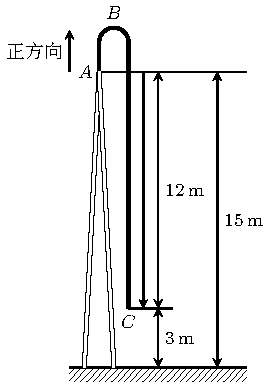
\includegraphics{fig/A/2-22.pdf}
    \caption{位移公式的应用}\label{fig_A_2-22}
\end{figure}


这个例题同学们也可以分上升运动和下降运动两步来计
算,所得结果是相同的.显然,这样分步计算比较麻烦.


\subsection*{练习十一}

\begin{enumerate}
	\item 在竖直上抛运动中,$v_t$与$v_0$何时方向相同,何时相反?$v_t$与$a$何时方向相同,何时相反?
\item 竖直向上射出的箭,初速度是35$\Ums$,上升的最大高度是多大?从射出到落回原地一共用多长时间?落回原地的速度是多大?
\item 竖直上抛的物体,初速度是30$\Ums$,经过2.0秒、3.0秒、4.0秒,物体的位移分别是多大?通过的路程分别是多长?各秒末的速度分别是多大?
\item 在课文的例题中,求经过1秒后石子离地面的高度以及石子这时的速度.先分上升运动和下降运动两步来计算,再用统一的公式来计算,并加以比较.
\end{enumerate}

\section*{复习题}

\begin{enumerate}
\item 什么是参照物?在研究物体的运动时为什么一定要选择参照物?

在什么情况下可以把物体看成质点?在什么情况下不能
把物体看成质点?
\item 什么是位移?位移和路程有什么区别?在什么情况下位移的大小等于路程?
\item 什么是匀速直线运动?什么是匀速直线运动的速度?匀速直线运动的位移公式是怎样的?利用位移公式,知道物体的初位置,又知道速度,能不能确定物体在任一时刻的位置?
\item 什么是变速直线运动?什么是变速直线运动的平均速度?什么是变速直线运动的即时速度?为什么测量平均速度的时间间隔足够短时,得出的平均速度就可以看做是即时速度?
\item 什么是匀变速直线运动?什么是匀变速直线运动的加速度?速度和加速度的区别是什么?
\item 匀变速直线运动的速度公式和位移公式是什么?利用这两个公式,知道物体的初位置和初速度,又知道加速度,能不能确定物体在任一时刻的位置和速度?
匀变速直线运动的两个有用的推论是什么?
\item 自由落体运动的加速度$g$有多大?怎样求出自由落体的下落速度和下落距离?
\item 已知竖直上抛物体的上抛速度$v_0$,怎样求出它的速度和位移?竖直上抛运动可以分上升运动和下降运动两步来计算,也可以用统一的公式来计算,哪种办法比较简便?
\item 匀速直线运动的位移图象是一条什么样的图线?怎样从这个图象求出物体的速度?

匀速直线运动的速度图象是一条什么样的图线?怎样从这个图象求出物体的位移?

匀变速直线运动的速度图象是一条什么样的图线?怎样从这个图象求出物体的位移?

\end{enumerate}


\section*{习题}
\begin{enumerate}
	\item 物体的加速度为零时,它的速度是否一定为零?物体的速度为零时,它的加速度是否一定为零?各举一个例子.
	\item 汽车以26$\Ukmh$的速度行驶了2小时,跟目的地还有一半路程,要想在40分钟内到达目的地,在后一半路程中汽车应该以多大速度行驶?
	\item 矿井里的升降机,从静止开始加速上升,经过3秒速度达到3$\Ums$,然后以这个速度匀速上升25秒,最后减速上升,经过2秒到达井口时,正好停下来,求矿井深度.
	\item 一架飞机以7.0$\Umsq$的加速度做匀加速飞行,计算它的速度由240$\Ukmh$增加到600$\Ukmh$所发生的位移和所用的时间.
	\item 火车制动后经过20秒停下来,在这段时间内前进120米.求火车开始制动时的速度和火车的加速度.
	\item 汽车从静止开始做匀变速运动,通过一段距离,速度达到14$\Ums$,汽车通过这段距离的一半时,速度是多大?
	\item 一个物体从塔顶上下落,在到达地面前最后一秒内通过的位移是整个位移的9/25,求塔高.
	\item 自由落下的物体在某一点速度是19.6$\Ums$,在另一点的速度是39.2$\Ums$.求这两点间的距离和经过这段距离所用的时间.
	\item 一个竖直上抛的物体,经过4.0秒落回原地,经过1.0秒,2.0秒,3.0秒,物体的速度分别是多大?物体的位移分别是多大?通过的路程分别是多长?
	\item 气球以10$\Ums$的速度匀速竖直上升,从气球上掉下一个物体,经17秒到达地面.求物体刚脱离气球时气球的高度.
	\item 初速度为零的匀变速运动,在第1秒内、第2秒内、第
	3秒内……的位移分别是$s_I,s_{II},s_{III},\ldots$.试证明:$s_I,s_{II},s_{III},\ldots$之比等于从1开始的连续奇数之比,即:
$$s_I:s_{II}:s_{III}\cdots=1:3:5\cdots$$

提示:设物体在1秒内、2秒内、3秒内……发生的位移是
$s_1 $,$ s_2 $,$ s_3 $,$ \cdots$,那么
$$s_I=s_1,   \quad  s_{II}=s_2-s_1,   \quad s_{III}=s_3-s_2,  \quad \cdots$$
	\item 从楼顶上落下一个铅球,通过1米高的窗子用了0.1秒的时间.楼顶比窗台高多少米?
\end{enumerate}





